\documentclass[a4paper, 11pt]{article}

\usepackage[utf8]{inputenc}

\usepackage[T1]{fontenc}

\usepackage[english]{babel}

\usepackage{graphicx}

\usepackage{multicol}

\usepackage{floatrow}

\usepackage[margin = 1in]{geometry}

\usepackage{float}

\usepackage[hidelinks, urlcolor=cyan]{hyperref}

\usepackage{url}

\usepackage{natbib}

\bibliographystyle{abbrvnat}
\setcitestyle{authoryear,open={(},close={)}}

\usepackage{csquotes}

\usepackage{fancyhdr}

%\addbibresource{references.bib}

\title{\Large BINF-402 Project \\
\huge Differential expression analysis of micro-RNA transcriptome between pancreas, prostate and gastrocnemius medialis tissues}


\author{Léopold Guyot}

\date{\today}

\begin{document}

\pagestyle{fancy}
\setlength{\headheight}{32.3pt}
\fancyhead{}\fancyfoot{}
\fancyhead[L]{
\includegraphics[width = 0.2\textwidth]{Figures/LOGO_Universite _libre_bruxelles.png}}
\fancyhead[R]{Differencial expression analysis of microRNA transcriptomes}
\fancyfoot[R]{\thepage}

\maketitle

\begin{multicols}{2}
\section{Introduction}
This analysis investigates microRNA expression variations across three distinct tissues; prostate gland, pancreas body, and gastrocnemius medialis. For this a simple workflow will be used, consisting of quality control of the reads, followed by a filtering, then a mapping to finish we a classic differential expression analysis. The goal is to unveil tissue-specific expression patterns of miRNA. Tissue selection is strategic, anticipating closer miRNA expression patterns between prostate and pancreas, both glandular, and unique signatures in gastrocnemius medialis, a muscle tissue.

\section{Methods}
All the data processing was done using the language R \citep{Rlang} and several packages. Note that for each section, the relevant scripts are indicated. Each script name is clickable to acces code through the associated github link. The link to the github repo is
{\scriptsize \href{https://github.com/leopoldguyot/BINF-402_Transcriptomic_Project/}{https://github.com/leopoldguyot/BINF-402\_Transcriptomic\_Project/}}
\subsection{Data Retrieval}
\begin{scriptsize}
	\textbf{Script associated : \href{https://github.com/leopoldguyot/BINF-402_Transcriptomic_Project/blob/main/retrieve_data.R}{retrieve\_data.R}}
\end{scriptsize}



All the data sets used in this project have been retrieve from the ENCODE database \citep{luo2020new}.
Three tissues have been selectionned; pancreas body, prostate gland and the gastrocnemius medialis tissue.
For each tissue, data used was coming from two distinct experiments, each comprising two replicates, thereby totaling four replicates per tissue (cf. \href{https://github.com/leopoldguyot/BINF-402_Transcriptomic_Project/blob/data/sample_table_links.csv}{"data/sample\_table\_links.csv"} for file accession numbers).

The original UCSC hg38 genome was used as reference for the mapping. The NCBI accession for this genome is \href{https://www.ncbi.nlm.nih.gov/datasets/genome/GCF_000001405.26/}{GCA\_000001405.26}.


\subsection{Read Quality Control}
\begin{scriptsize}
	 \textbf{Scripts associated : \href{https://github.com/leopoldguyot/BINF-402_Transcriptomic_Project/blob/main/reads_mapping.R}{reads\_mapping.R},\\
	 	  \href{https://github.com/leopoldguyot/BINF-402_Transcriptomic_Project/blob/main/Quality_control_stats.R}{Quality\_control\_stats.R}, \\
	 	  \href{https://github.com/leopoldguyot/BINF-402_Transcriptomic_Project/blob/main/quality_control.R}{quality\_control.R}}
\end{scriptsize}


A preliminary analysis done using the Rqc package \citep{Rqc} revealed notable issues with the quality of the sequencing reads. Others statistics have been retrieve and used to find the problems and adapt the processing of the reads. 

Red line in the summary Figure \ref{fig:cycles_mean} depict the evolution of the quality trough the cycles for the unprocessed reads, indicate a substantial low mean quality for the initial 5 cycles and a significant decrease from the 43rd cycle to the end of the reads (mean quality of the cycles of unprocessed reads is highlighted by the red line in the figure).

To address these quality issues, an initial processing step was implemented using the QuasR package \citep{QuasR} (for performance reasons). This step involved trimming the first 5 and the last 7 cycles of the reads (additionally, reads with unidentified residues were filtered out). The result is visible with the green line in Figure \ref{fig:cycles_mean}. Even after this first step, a persistent decrease in mean quality throughout the remaining cycles was still observed.

In response to the persistent decline in mean quality, a second processing step was undertaken. In this step, reads were filtered to retain only those with a mean quality higher than 20. The outcome of this filtering is illustrated by the blue line in Figure \ref{fig:cycles_mean}. This additional processing step led to a global increase in mean quality across the entire read length and a stable read quality through cycles, the previous trend of decreasing quality has been effectively mitigated.


\begin{figure}[H]
    \centering
    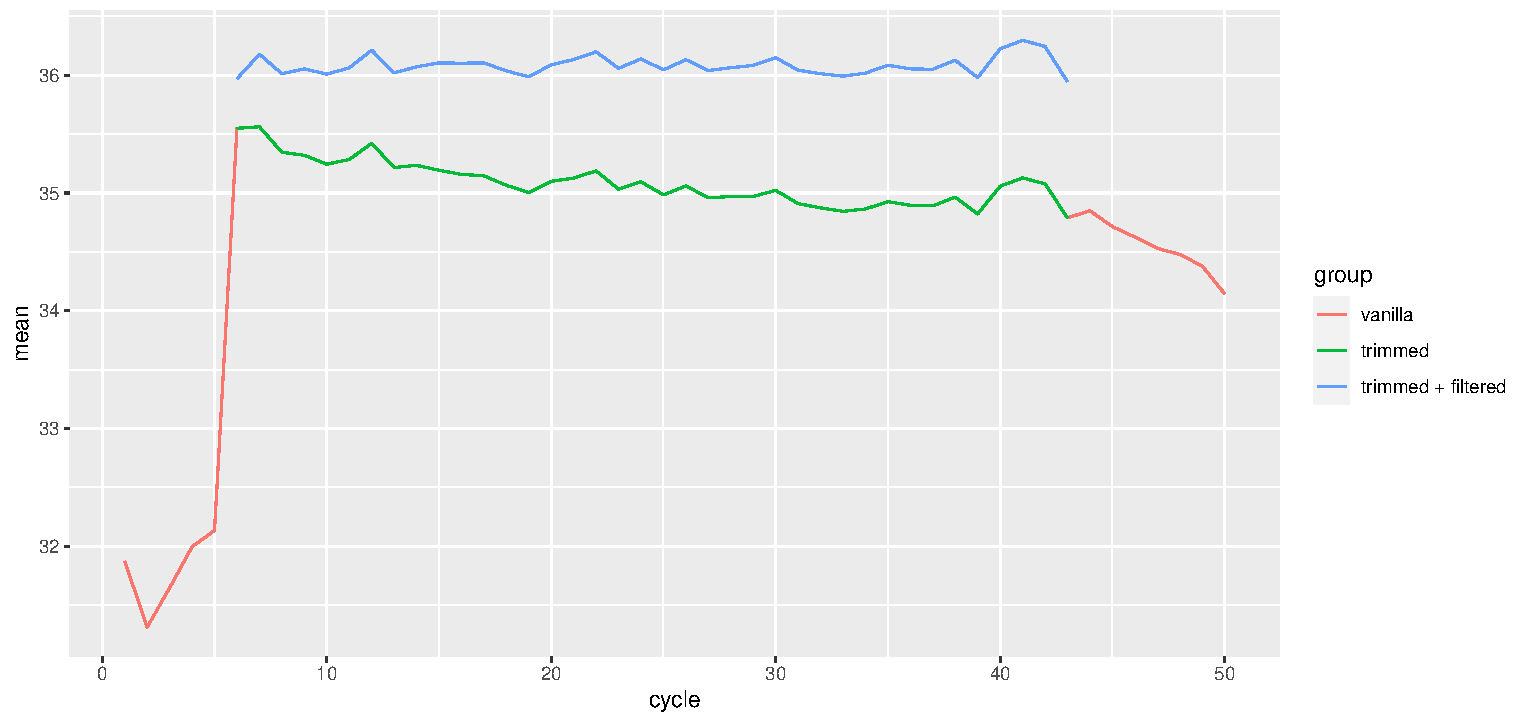
\includegraphics[width=1\columnwidth]{Figures/QC_plots/mean_per_group_and_cycles.pdf}
    \caption{\small{ Graph of the mean quality for each cycle.}}
    \label{fig:cycles_mean}
\end{figure}

In the following section, the mapping performance for each version of the data (unprocessed, with trimming, with trimming and filtering) will be explored. This analysis will provide insights into how the quality enhancements impact the alignment of reads.

\subsection{Mapping}
\begin{scriptsize}
	\textbf{Script associated : \href{https://github.com/leopoldguyot/BINF-402_Transcriptomic_Project/blob/main/reads_mapping.R}{reads\_mapping.R}} 
\end{scriptsize}

present mapping stats
\begin{figure}[H]
    \centering
    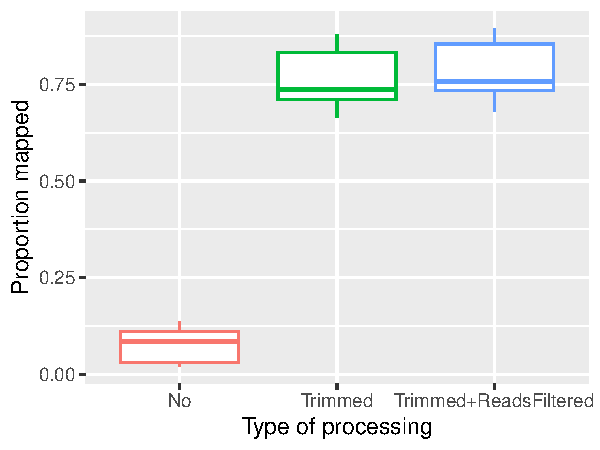
\includegraphics[width=1\columnwidth]{Figures/mapping_props.pdf}
    \caption{Caption of the figure.}
    \label{fig:mapping}
\end{figure}
\subsection{Differential Expression Analysis}
\begin{scriptsize}
	\textbf{Script associated : \href{https://github.com/leopoldguyot/BINF-402_Transcriptomic_Project/blob/main/differential_expression_analysis.R}{differential\_expression\_analysis.R}} 
\end{scriptsize}

%\subsection{Gene Ontology}

\section{Results}

Present the overall results => Differential Expression Analysis


\section{Discussion}
???? maybe not include it
=> things I could Improve


\section{Conclusion}


\bibliography{references}

\end{multicols}
\end{document}
